%%%%%%%%%%%%%%%%%%%%%%%%%%%%%%%%%%%%%%%%%%%%%%%%%%%%%%%%%%%%%%%%%%%%%%%%%%
%
% Plantilla para libro de texto de matemáticas.
%
% Esta plantilla ha sido desarrollada desde cero, pero utiliza algunas partes
% del código de la plantilla original utilizada en apuntesDGIIM
% (https://github.com/libreim/apuntesDGIIM), basada a su vez en las plantillas
% 'Short Sectioned Assignment' de Frits Wenneker (http://www.howtotex.com),
% 'Plantilla de Trabajo' de Mario Román y 'Plantilla básica de Latex en Español'
% de Andrés Herrera Poyatos (https://github.com/andreshp). También recoge
% ideas de la plantilla 'Multi-Purpose Large Font Title Page' de
% Frits Wenneker y Vel (vel@latextemplates.com).
%
% Licencia:	
% CC BY-NC-SA 4.0 (https://creativecommons.org/licenses/by-nc-sa/4.0/)
%
%%%%%%%%%%%%%%%%%%%%%%%%%%%%%%%%%%%%%%%%%%%%%%%%%%%%%%%%%%%%%%%%%%%%%%%%%

% ---------------------------------------------------------------------------
% CONFIGURACIÓN BÁSICA DEL DOCUMENTO
% ---------------------------------------------------------------------------

%\documentclass[11pt, a4paper, twoside]{article} % Usar para imprimir
\documentclass[10pt, a4paper]{article}

\linespread{1.3}            % Espaciado entre líneas.
\setlength\parindent{0pt}   % No indentar el texto por defecto.
\setlength\parskip{7pt}

% ---------------------------------------------------------------------------
% PAQUETES BÁSICOS
% ---------------------------------------------------------------------------

% IDIOMA
\usepackage[utf8]{inputenc}
\usepackage[spanish, es-tabla, es-lcroman, es-noquoting]{babel}
\usepackage[table,xcdraw]{xcolor}

% MATEMÁTICAS
\usepackage{amsmath}    % Paquete básico de matemáticas
\usepackage{amsthm}     % Teoremas
\usepackage{mathrsfs}   % Fuente para ciertas letras utilizadas en matemáticas

% FUENTES
\usepackage{newpxtext, newpxmath}   % Fuente similar a Palatino
\usepackage{FiraSans}                 % Fuente sans serif
\usepackage[T1]{fontenc}
\usepackage[italic]{mathastext}     % Utiliza la fuente del documento
                                    % en los entornos matemáticos

% MÁRGENES
\usepackage[margin=2.5cm, top=3cm]{geometry}

% LISTAS
\usepackage{enumitem}       % Mejores listas
\setlist{leftmargin=.5in}   % Especifica la indentación para las listas.

% Listas ordenadas con números romanos (i), (ii), etc.
\newenvironment{nlist}
{\begin{enumerate}
    \renewcommand\labelenumi{(\emph{\roman{enumi})}}}
  {\end{enumerate}}

%  OTROS
\usepackage[hidelinks]{hyperref}   % Enlaces
\usepackage{graphicx}   % Permite incluir gráficos en el documento
\usepackage{relsize}

% LISTINGS
\usepackage{listings}
\usepackage{xcolor}     % Permite definir y utilizar colores
\usepackage{lipsum}
\usepackage{courier}

% Fijar tabla a posición
\usepackage{array}
\newcolumntype{L}[1]{>{\raggedright\let\newline\\\arraybackslash\hspace{0pt}}m{#1}}
\newcolumntype{C}[1]{>{\centering\let\newline\\\arraybackslash\hspace{0pt}}m{#1}}
\newcolumntype{R}[1]{>{\raggedleft\let\newline\\\arraybackslash\hspace{0pt}}m{#1}}


% Colores para los bloques de código
\definecolor{codegreen}{rgb}{0,0.6,0}
\definecolor{codegray}{rgb}{0.5,0.5,0.5}
\definecolor{codepurple}{rgb}{0.58,0,0.82}
\definecolor{backcolour}{rgb}{0.95,0.95,0.92}
\lstdefinestyle{mystyle}{
	backgroundcolor=\color{backcolour},   
	commentstyle=\color{codegreen},
	keywordstyle=\color{blue},
	numberstyle=\tiny\color{codegray},
	stringstyle=\color{codepurple},
	basicstyle=\footnotesize\ttfamily,
	breakatwhitespace=false,         
	breaklines=true,                 
	captionpos=b,                    
	keepspaces=true,                 
	numbers=left,                    
	numbersep=5pt,                  
	showspaces=false,                
	showstringspaces=false,
	showtabs=false,                  
	tabsize=4
}
\lstset{style=mystyle}

%\lstset{basicstyle=\footnotesize\ttfamily,breaklines=true}
%\lstset{framextopmargin=50pt,frame=bottomline}
 
% ---------------------------------------------------------------------------
% COMANDOS PERSONALIZADOS
% ---------------------------------------------------------------------------

% \equalto
\newcommand{\verteq}{\rotatebox{90}{$\,=$}}
\newcommand{\equalto}[2]{\underset{\scriptstyle\overset{\mkern4mu\verteq}{#2}}{#1}}


% ---------------------------------------------------------------------------
% COLORES
% ---------------------------------------------------------------------------

\definecolor{50}{HTML}{E0F2F1}
\definecolor{100}{HTML}{B2DFDB}
\definecolor{200}{HTML}{80CBC4}
\definecolor{300}{HTML}{4DB6AC}
\definecolor{400}{HTML}{26A69A}
\definecolor{500}{HTML}{009688}
\definecolor{600}{HTML}{00897B}
\definecolor{700}{HTML}{00796B}
\definecolor{800}{HTML}{00695C}
\definecolor{900}{HTML}{004D40}

% ---------------------------------------------------------------------------
% DISEÑO DE PÁGINA
% ---------------------------------------------------------------------------

\usepackage{pagecolor}
\usepackage{afterpage}

% ---------------------------------------------------------------------------
% CABECERA Y PIE DE PÁGINA
% ---------------------------------------------------------------------------

\usepackage{fancyhdr}   % Paquete para cabeceras y pies de página

% Indica que las páginas usarán la configuración de fancyhdr
\pagestyle{fancy}
\fancyhf{}

% Representa la sección de la cabecera
\renewcommand{\sectionmark}[1]{%
\markboth{#1}{}}

% Representa la subsección de la cabecera
\renewcommand{\subsectionmark}[1]{%
\markright{#1}{}}

% Parte derecha de la cabecera
\fancyhead[LE,RO]{\sffamily\textsl{\rightmark} \hspace{1em}  \textcolor{500}{\rule[-0.4ex]{0.2ex}{1.2em}} \hspace{1em} \thepage}

% Parte izquierda de la cabecera
\fancyhead[RE,LO]{\sffamily{\leftmark}}

% Elimina la línea de la cabecera
\renewcommand{\headrulewidth}{0pt}

% Controla la altura de la cabecera para que no haya errores
\setlength{\headheight}{14pt}

% ---------------------------------------------------------------------------
% TÍTULOS DE PARTES Y SECCIONES
% ---------------------------------------------------------------------------

\usepackage{titlesec}

% Estilo de los títulos de las partes
\titleformat{\part}[hang]{\Huge\bfseries\sffamily}{\thepart\hspace{20pt}\textcolor{500}{|}\hspace{20pt}}{0pt}{\Huge\bfseries}
\titlespacing*{\part}{0cm}{-2em}{2em}[0pt]

% Reiniciamos el contador de secciones entre partes (opcional)
\makeatletter
\@addtoreset{section}{part}
\makeatother

% Estilo de los títulos de las secciones, subsecciones y subsubsecciones
\titleformat{\section}
  {\Large\bfseries\sffamily}{\thesection}{0em}{}

\titleformat{\subsection}
  {\Large\sffamily}{\thesubsection}{1em}{}[\vspace{.5em}]

\titleformat{\subsubsection}
  {\sffamily}{\thesubsubsection}{1em}{}

% CAMBIO DE NUMERACIÓN - ESPECÍFICO DE ESTE DOCUMENTO
\renewcommand{\thesection}{}
\renewcommand{\thesubsection}{\arabic{subsection}}

% ---------------------------------------------------------------------------
% ENTORNOS PERSONALIZADOS
% ---------------------------------------------------------------------------

\usepackage{mdframed}

%% DEFINICIONES DE LOS ESTILOS

% Nuevo estilo para definiciones
\newtheoremstyle{definition-style}  % Nombre del estilo
{}                                  % Espacio por encima
{}                                  % Espacio por debajo
{}                                  % Fuente del cuerpo
{}                                  % Identación
{\bf\sffamily}                      % Fuente para la cabecera
{.}                                 % Puntuación tras la cabecera
{.5em}                              % Espacio tras la cabecera
{\thmname{#1}\thmnumber{ #2}\thmnote{ (#3)}}  % Especificación de la cabecera

% Nuevo estilo para notas
\newtheoremstyle{remark-style}
{10pt}
{10pt}
{}
{}
{\itshape \sffamily}
{.}
{.5em}
{}

% Nuevo estilo para teoremas y proposiciones
\newtheoremstyle{theorem-style}
{}
{}
{}
{}
{\bfseries \sffamily}
{.}
{.5em}
{\thmname{#1}\thmnumber{ #2}\thmnote{ (#3)}}

% Nuevo estilo para ejemplos
\newtheoremstyle{example-style}
{10pt}
{10pt}
{}
{}
{\bf \sffamily}
{}
{.5em}
{\thmname{#1}\thmnumber{ #2.}\thmnote{ #3.}}

% Nuevo estilo para la demostración

\makeatletter
\renewenvironment{proof}[1][\proofname] {\par\pushQED{\qed}\normalfont\topsep6\p@\@plus6\p@\relax\trivlist\item[\hskip\labelsep\itshape\sffamily#1\@addpunct{.}]\ignorespaces}{\popQED\endtrivlist\@endpefalse}
\makeatother

%% ASIGNACIÓN DE LOS ESTILOS

% Teoremas, proposiciones y corolarios
\newtheoremstyle{theorem-style}{}{}{}{}{}{}{ }{}
\theoremstyle{theorem-style}
\newtheorem*{datos}{}
\theoremstyle{theorem-style}
\newtheorem{nth}{Teorema}[section]
\newtheorem{nprop}{Proposición}[section]
\newtheorem{ncor}{Corolario}[section]
\newtheorem{lema}{Lema}[section]

% Definiciones
\theoremstyle{definition-style}
\newtheorem{ndef}{Definición}[section]

% Notas
\theoremstyle{remark-style}
\newtheorem*{nota}{Nota}

% Ejemplos
\theoremstyle{example-style}
\newtheorem{ejemplo}{Ejemplo}[section]

% Ejercicios y solución
\theoremstyle{definition-style}
\newtheorem{ejer}{Ejercicio}[section]

\theoremstyle{remark-style}
\newtheorem*{sol}{Solución}

%% MARCOS DE LOS ESTILOS

% Configuración general de mdframe, los estilos de los teoremas, etc
\mdfsetup{
  skipabove=1em,
  skipbelow=1em,
  innertopmargin=1em,
  innerbottommargin=1em,
  splittopskip=2\topsep,
}

% Definimos los marcos de los estilos


\mdfdefinestyle{datos-frame}{
	linewidth=2pt, %
	linecolor= 500, %
	topline=false, %
	bottomline=false, %
	rightline=false,%
	leftmargin=0em, %
	innerleftmargin=1em, %
	innerrightmargin=1em,
	rightmargin=0em, %
}%
\mdfdefinestyle{nth-frame}{
	linewidth=2pt, %
	linecolor= 500, %
	topline=false, %
	bottomline=false, %
	rightline=false,%
	leftmargin=0em, %
	innerleftmargin=1em, %
  innerrightmargin=1em,
	rightmargin=0em, %
}%

\mdfdefinestyle{nprop-frame}{
	linewidth=2pt, %
	linecolor= 300, %
	topline=false, %
	bottomline=false, %
	rightline=false,%
	leftmargin=0pt, %
	innerleftmargin=1em, %
	innerrightmargin=1em,
	rightmargin=0pt, %
}%

\mdfdefinestyle{ndef-frame}{
	linewidth=2pt, %
	linecolor= 500, %
	backgroundcolor= 50,
	topline=false, %
	bottomline=false, %
	rightline=false,%
	leftmargin=0pt, %
	innerleftmargin=1em, %
	innerrightmargin=1em,
	rightmargin=0pt, %
}%

\mdfdefinestyle{ejer-frame}{
	linewidth=2pt, %
	linecolor= 300, %
	backgroundcolor= 50,
	topline=false, %
	bottomline=false, %
	rightline=false,%
	leftmargin=0pt, %
	innerleftmargin=1em, %
	innerrightmargin=1em,
	rightmargin=0pt, %
}%

\mdfdefinestyle{ejemplo-frame}{
	linewidth=0pt, %
	linecolor= 300, %
	leftline=false, %
	rightline=false, %
	leftmargin=0pt, %
	innerleftmargin=1.3em, %
	innerrightmargin=1em,
	rightmargin=0pt, %
	innertopmargin=0em,%
	innerbottommargin=0em, %
	splittopskip=\topskip, %
}%

% Asignamos los marcos a los estilos
\surroundwithmdframed[style=nth-frame]{nth}
\surroundwithmdframed[style=datos-frame]{datos}
\surroundwithmdframed[style=nprop-frame]{nprop}
\surroundwithmdframed[style=nprop-frame]{ncor}
\surroundwithmdframed[style=ndef-frame]{ndef}
\surroundwithmdframed[style=ejer-frame]{ejer}
\surroundwithmdframed[style=ejemplo-frame]{ejemplo}
\surroundwithmdframed[style=ejemplo-frame]{sol}

% ---------------------------------------------------------------------------
% CONFIGURACIÓN DE LA PORTADA
% ---------------------------------------------------------------------------

\newcommand{\asignatura}{Análisis de eficiencia de algoritmos}

\newcommand{\autor}{Celia Arias Martínez\\Miguel Ángel Fernández Gutiérrez\\Sergio Quijano Rey\\Lucía Salamanca López\\\hspace{1cm}}

\newcommand{\grado}{segfault}

\newcommand{\universidad}{Universidad de Granada}

\newcommand{\enlaceweb}{github.com/DGIIMUnderground}

% ---------------------------------------------------------------------------
% CONFIGURACIÓN PERSONALIZADA
% ---------------------------------------------------------------------------

%%%%%%%%%%%%%%%%%%%%%%%%%%%%%%%%%%%%%%%%%%%%%%%%%%%%%%%%%%%%%%%%%%%%%%%%%%%%%
% ---------------------------------------------------------------------------
% COMIENZO DEL DOCUMENTO
% ---------------------------------------------------------------------------
%%%%%%%%%%%%%%%%%%%%%%%%%%%%%%%%%%%%%%%%%%%%%%%%%%%%%%%%%%%%%%%%%%%%%%%%%%%%%

\begin{document}

% ---------------------------------------------------------------------------
% PORTADA EXTERIOR
% ---------------------------------------------------------------------------

\newpagecolor{500}\afterpage{\restorepagecolor} % Color de la página
\begin{titlepage}

  % Título del documento
	\parbox[t]{\textwidth}{
			\raggedright % Texto alineado a la izquierda
			\fontsize{40pt}{40pt}\selectfont\sffamily\color{white}{
				\textbf{\Huge{Práctica 4}}\\\textbf{Programación dinámica }\\\huge{Algorítmica}
      }
	}

	\vfill

	%% Autor e información del documento
	\parbox[t]{\textwidth}{
		\raggedright % Texto alineado a la izquierda
		\sffamily\large\color{white}
		\grado\\
		{\Large \autor }\\[15pt]
		
\includegraphics[width=130pt]{ugrlogo.pdf}
	}

\end{titlepage}

% ---------------------------------------------------------------------------
% PÁGINA DE LICENCIA
% ---------------------------------------------------------------------------

\thispagestyle{empty}
\null
\vfill

%% Información sobre la licencia
\parbox[t]{\textwidth}{
  
\includegraphics{by-nc-sa.pdf}\\[4pt]
  \raggedright % Texto alineado a la izquierda
  \sffamily\large
  {\Large Este trabajo se distribuye bajo una licencia CC BY-NC-SA 4.0.}\\[4pt]
  Eres libre de distribuir y adaptar el material siempre que reconozcas a los\\
  autores originales del documento, no lo utilices para fines comerciales\\
  y lo distribuyas bajo la misma licencia.\\[4pt]
  \texttt{creativecommons.org/licenses/by-nc-sa/4.0/}
}

% ---------------------------------------------------------------------------
% PORTADA INTERIOR
% ---------------------------------------------------------------------------

\begin{titlepage}

  % Título del documento
  \parbox[t]{\textwidth}{
  	\raggedright % Texto alineado a la izquierda
  	\fontsize{40pt}{40pt}\selectfont\sffamily\color{500}{
  		\textbf{\Huge{Práctica 4}}\\\textbf{Programación dinámica}\\\huge{Algorítmica}
  	}
  }

	\vfill
	
	%% Autor e información del documento
	\parbox[t]{\textwidth}{
		\raggedright % Texto alineado a la izquierda
		\sffamily\large
		\grado\\
		{\Large \autor }\\[15pt]
		
\includegraphics[width=130pt]{ugrlogo-dark.pdf}
	}

\end{titlepage}

% ---------------------------------------------------------------------------
% ÍNDICE
% ---------------------------------------------------------------------------

\thispagestyle{empty}
\tableofcontents
\newpage

% ---------------------------------------------------------------------------
% CONTENIDO
% ---------------------------------------------------------------------------

\part{Introducción}

En la \textbf{práctica 4}, de programación dinámica, teníamos que elegir entre los dos problemas propuestos: 

\begin{itemize}
	\item \textbf{Viajante de comercio:} dado un conjunto de ciudades y una matriz con las distancias entre ellas encontrar el camino más corto que las recorra todas una vez.
	\item \textbf{Subsecuencia de caracteres más larga:} encontrar la máxima subsecuencia de caracteres comunes.  
\end{itemize}
Nosotros hemos decidido estudiar el segundo problema.

\subsection*{Objetivo de esta práctica}

En esta práctica, pretenderemos apreciar la utilidad de los algoritmos de programación dinámica para encontrar la solución óptima en problemas que podemos dividir en subproblemas superpuestos.

Para ello, daremos una solución al problema de la \emph{subsecuencia de caracteres más larga} y compararemos la eficiencia de este algoritmo respecto al algoritmo de \emph{fuerza bruta} y \emph{recurrencias}.

\pagebreak
\part{Desarrollo}

\section{Máxima subsecuencia de caracteres (LCS)}

\begin{datos}
	{\sffamily Dadas dos secuencias de caracteres, encontrar la máxima subsecuencia de caracteres común que aparecen en ambas cadenas de izquierda a derecha (no necesariamente de forma contigua).}
\end{datos}


\subsection{Enfoque por programación dinámica}

Aplicamos programación dinámica en cuatro fases:

\begin{enumerate}
	\item Verificación de la naturaleza $n$-etápica del problema.
	\item Verificación del principio de optimalidad de Bellman.
	\item Planteamiento de una recurrencia. 
	\item Cálculo de la solución.
\end{enumerate}


\subsubsection{Naturaleza n-etápica}

El resultado es consecuencia de una sucesión de decisiones: en la etapa $n$ debemos elegir qué cadena de caracteres dejamos fija y qué puntero movemos hacia la derecha. 

Una solución optimal de decisiones será aquella que maximice la función objetivo, es decir, aquella que proporcione la subsecuencia de caracteres más larga.

\subsubsection{Verificación del principio de optimalidad de Bellman}

El \textbf{principio de optimalidad de Bellman (POB)}, es una condición necesaria para la optimalidad en programación dinámica. 

Tenemos que escribir el valor del problema en la etapa $n$ en función de los valores en la etapa 1 y las decisiones óptimas tomadas en las etapas anteriores. De esta forma conseguimos obtener subproblemas más simples, ya que no tendremos que volver a calcular todas las soluciones, pues tenemos asegurado que utilizamos solo las óptimas.  
 
En nuestro problema la función a maximizar es el número de caracteres en común en las dos subsecuencias. Tendremos, por tanto, en la etapa $n$:
$$
	f_n(i,j) = \text{máx}\{f(i-1,j),f(i,j-1)\}+\delta_{ij}
$$
donde $\delta_{ij}$ es la función que dados dos índices, cada uno respectivo a una subcadena, devuelve uno si coinciden y cero en caso contrario.

El caso base es:
$$
	f_1(i,j) = \text{máx}\{\delta_{ij}\} = \delta_{ij}
$$
Es obvio que la solución proporcionada en la etapa $n$ es optimal, pues estamos calculando el máximo de dos funciones optimales. De igual forma, si $f_{n-1}(i-1,j)$ ó $f_{n-1}(i,j-1)$ no son optimales en el paso anterior hubiéramos calculado $f'_{n-1}(i-1,j)$ ó $f'_{n-1}(i,j-1)$.

Por tanto, podemos decir que el problema cumple el principio de optimalidad de Bellman. 

\subsubsection{Planteamiento de recurrencia}
La recurrencia planteada ha sido la siguiente:


$$ LCS{[i,j]}= \left\{\begin{matrix} 1+LCS[i-1,j-1] \\ \text{máx}\{LCS[i-1,j],LCS[i,j-1]\})\end{matrix}\right. $$

Si encontramos dos caracteres que coincidan aumentamos en uno el tamaño de la solución parcial que tenemos y llamamos a la función moviendo a la izquierda los dos punteros. Si no coinciden volvemos a llamar a la función moviendo el puntero una posición a la izquierda sobre la cadena primera, y después volvemos a llamarla moviendo el puntero de la segunda cadena. De los valores obtenidos cogemos siempre el máximo.

De esta forma conseguimos asegurar el principio de optimalidad: si estamos en la etapa $n$, las decisiones tomadas hasta la etapa $n-1$ son óptimas.


\subsubsection{Cálculo de la solución}

Para ello, hemos planteado el siguiente algoritmo:

\begin{lstlisting}[language=C]
vector<vector<int> > constructLCSMat(string str1, string str2) {
	vector<vector<int> > lcs_mat(str1.size() + 1, vector<int>(str2.size() + 1, 0));
	
	for ( int i = 1; i <= str1.size(); i++ ) {
		for ( int j = 1; j <= str2.size(); j++ ) {
			if ( str1[i-1] == str2[j-1] )
				lcs_mat[i][j] = 1 + lcs_mat[i-1][j-1];
			else
				lcs_mat[i][j] = max(lcs_mat[i-1][j], lcs_mat[i][j-1]);
		}
	}
	
	return lcs_mat;
}
\end{lstlisting}
\pagebreak
\begin{lstlisting}[language=C]
string getLCS(string str1, string str2) {
	vector<vector<int> > lcs_mat = constructLCSMat(str1, str2);
	string word;
	
	int i = str1.size(), j = str2.size();
	
	while ( j > 0 ) {
		j--;
		if ( lcs_mat[i][j] != lcs_mat[i][j+1] ) {
			word = str2[j] + word;
			i--;
		}
	}
	
	return word;
}
\end{lstlisting}

En el que utilizamos las siguientes funciones y estructuras de datos:

\begin{itemize}
	\item Una función \textbf{\texttt{constructLCSMat}}, donde creamos la matriz que utilizaremos para encontrar el número de caracteres y las letras que conforman la máxima subsecuencia en común. Con dos bucles \texttt{for} anidados recorremos las dos palabras, comprobando si coinciden las letras y consultando los datos de la matriz ya escritos anteriormente, como podemos ver en la recurrencia especificada antes.

	Cuando la matriz esté calculada, la devolvemos. Esta matriz será usada por la función \texttt{getLCS}.
	\item La función \textbf{\texttt{getLCS}}, que recibe como argumentos las dos palabras estudiadas. Dentro llamamos a la función \texttt{constructLCSMat} para construir la matriz. Con el bucle \texttt{while} recorremos la matriz de derecha a izquierda por filas, empezando por la última fila y la última columna: cuando veamos que el valor respecto a la columna anterior cambia, subimos de fila y guardamos la letra que corresponda a esa posición, ya que significará que hemos sumado uno, y por tanto que los valores en la palabra de $i$ y $j$ coinciden.
\end{itemize}
\pagebreak
\subsubsection{Un ejemplo ilustrativo}

Para ilustrar lo que hacen nuestras funciones, tomamos como ejemplo las secuencias de caracteres:
$$\text{\texttt{str1}=``ropero''\hspace{2cm}\texttt{str2}=``armario''}$$

Evidentemente, la solución es \textbf{``rro''}.

\begin{center}
	
\includegraphics[width=5cm]{./resources/diagrama.png}
\end{center}

\vspace{0.5cm}
La función \texttt{getLCS} llamaría en primer lugar, a \texttt{constructLCSMat}, que generaría la siguiente matriz:

$$
\begin{matrix}
 & \begin{matrix} \textcolor{white}{....}\vspace{0.3cm}&\text{{a}} & \text{{r}} & \text{{m}} & \text{{a}} & \text{{r}} & \text{{i}} & \text{{o}} \end{matrix} \\
\begin{matrix}\\ \text{{r}}\\\text{{o}}\\\text{{p}}\\\text{{e}}\\\text{{r}}\\\text{{o}} \end{matrix} & \left(\begin{matrix}
0 & 0 & 0 &0&0&0&0&0\\
0&0&1&1&1&1&1&1\\
0&0&1&1&1&1&1&2\\
0&0&1&1&1&1&1&2\\
0&0&1&1&1&1&1&2\\
0&0&1&1&1&2&2&2\\
0&0&1&1&1&2&2&3\\
\end{matrix}\right)
\end{matrix}
$$

Esta matriz, será procesada en \texttt{getLCS}. En su recorrido, obtendremos la subsecuencia más corta:

$$
\begin{matrix}
 & \begin{matrix} \textcolor{white}{....}\vspace{0.3cm}&\text{{a}} & \text{\textcolor{red}{r}} & \text{{m}} & \text{{a}} & \text{\textcolor{red}{r}} & \text{{i}} & \text{\textcolor{red}{o}} \end{matrix} \\
\begin{matrix}\\ \text{\textcolor{red}{r}}\\\text{{o}}\\\text{{p}}\\\text{{e}}\\\text{\textcolor{red}{r}}\\\text{{\textcolor{red}{o}}} \end{matrix} & \left(\begin{matrix}
0 & 0 & 0 &0&0&0&0&0\\
0&0&\textbf{\textcolor{red}{1}}&1&1&1&1&1\\
0&0&\textbf{1}&1&1&1&1&2\\
0&0&\textbf{1}&1&1&1&1&2\\
0&0&\textbf{1}&\textbf{1}&\textbf{1}&1&1&2\\
0&0&1&1&1&\textbf{\textcolor{red}{2}}&\textbf{2}&2\\
0&0&1&1&1&2&2&\textbf{\textcolor{red}{3}}\\
\end{matrix}\right)
\end{matrix}
$$

Teniendo como resultado la subsecuencia ``rro'' (\textbf{r}ope\textbf{ro}, a\textbf{r}ma\textbf{r}i\textbf{o}).

\pagebreak
\subsection{Análisis empírico}

Para el análisis de tiempo, hemos creado un código que ejecute, sobre un mismo conjunto de datos aleatorio, dos algoritmos: \texttt{dynamic}, el explicado anteriormente (que hace uso de programación dinámica) y \texttt{brute}, por fuerza bruta usando la recursividad, directamente.

Los tamaños de prueba para ejecutar el algoritmo han sido:
\begin{itemize}
	\item desde 500 hasta 3600 en saltos de 500
	\item desde 3600 hasta 56000 en saltos de 10000.
	\item hasta 49000 en saltos de 1000.
\end{itemize}

A su vez cada iteración la hemos hecho 100 veces y hemos calculado la media, con el fin de eliminar los mejores y peores casos.

\begin{datos}
	{\bf\sffamily Gráfico 2.1.} {\sffamily Datos empíricos: algoritmo dinámico}\\
	\vspace{-0.7cm}
	\begin{center}
		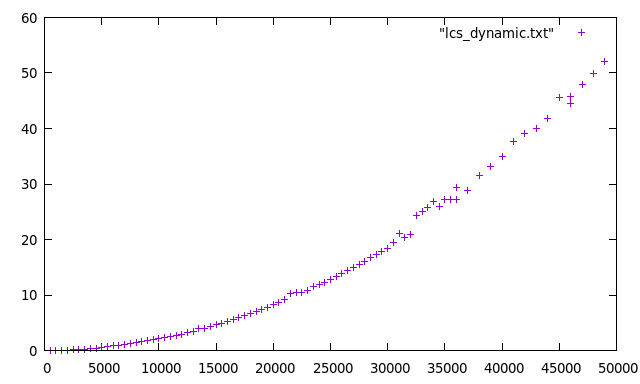
\includegraphics[width=15cm]{./../Graficas/lcs_dinamic.png}
	\end{center}	
\end{datos}

Los datos de las gráficas se encuentran en la \textbf{\emph{sección IV: Anexo I}} de este documento.

Podemos decir que la gráfica crece de forma cuadrática, por lo que podemos ejecutarlo para valores suficientemente grandes. Esto se debe que tenemos que generar la matriz, que es de complejidad O($n^2$). Puede parecer una complejidad alta, pero comparada con el coste de llamar a la función recursivamente es aceptable. Probaremos lo dicho empíricamente en la sección siguiente.

\subsection{Comparación de enfoques}

Hemos comparado nuestro algoritmo con un algoritmo de  \emph{recurrencia} simple. Como \emph{recurrencia} solo funciona para tamaños muy pequeños hemos recogido datos con $n = 17$.

Podemos observar en el {\sffamily gráfico 6.2} que a partir de $n=13$ se aprecia una diferencia notable en los tiempos de ejecución: con estos valores nuestro algoritmo parece que se mantiene constante mientras que el algoritmo de fuerza bruta, por recurrencia, crece exponencialmente.

\begin{datos}
	{\bf\sffamily Gráfico 3.1.} {\sffamily Contraste de datos empíricos: algoritmo dinámico vs. fuerza bruta}\\
	\vspace{-0.7cm}
	\begin{center}
		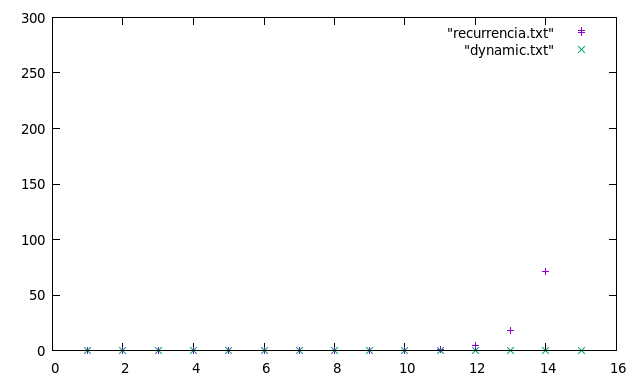
\includegraphics[width=15cm]{../Graficas/comparacion.png}
	\end{center}	
\end{datos}
\pagebreak
\part{Conclusiones}

Con esta práctica, hemos aprendido a crear algoritmos de programación dinámica para resolver problemas encadenados que podemos optimizar. 

Hemos comprobado las cuatro condiciones que tiene que reunir un problema para poder resolverse con programación dinámica. 

Así mismo, hemos observado la utilidad de este tipo de algoritmos: al contrario de algoritmos simples de recurrencia en cada iteración no hay que volver a comprobar todas las soluciones posibles, ya que hemos guardado las mejores soluciones anteriores (en este caso, en una tabla o matriz).

Esto es de especial relevancia en los que queremos encontrar la solución óptima tomando una serie de decisiones: el tiempo será peor que en algoritmos \emph{greedy}, sin embargo nos aseguramos de que la solución proporcionada es la mejor.


\pagebreak

\part{Anexos}

\section*{Anexo I. Códigos}

\subsubsection*{Programación dinámica: \texttt{lcs\_dynamic.hpp}}
\begin{lstlisting}[language=C]
/**
 * @brief Longest Common Subsequence: encontrar subcadena mas larga - Programacion Dinamica
 * @file lcs_dynamic.cpp
 * @author segfault
 */
#include <vector>
#include <string>
#include <iostream>

using namespace std;


namespace dynamic {

    /**
     * @brief Calcula el maximo de dos enteros
     * @param a: uno
     * @param b: el otro
     * @return el maximo de ambos
     */
    int max(int a, int b) {
        if (a > b)
            return a;
        else
            return b;
    }

    /**
     * @brief Funcion para imprimir la matriz LCS, incluyendo caracteres
     * @param mat: matriz LCS
     * @param str1: primera palabra
     * @param str2: segunda palabra
     */
    void printmat(vector<vector<int> > mat, string str1, string str2) {
        // cabecera: segunda palabra
        cout << "    ";
        for ( int i = 0; i < str2.size(); i++ )
            cout << str2[i] << ' ';
        cout << endl;

        for ( int i = 0; i < mat.size(); i++ ) {
            // primera palabra
            if ( i == 0 )
                cout << "  ";
            else
                cout << str1[i-1] << ' ';

            // imprimir elementos de la matriz
            for ( int j = 0; j < mat[0].size(); j++ )
                cout << mat[i][j] << " ";

            cout << endl;
        }
    }

    /**
     * @brief Crea la matriz LCS
     * @param str1: primera palabra
     * @param str2: segunda palabra
     * @return matriz LCS de las palabras str1, str2
     */
    vector<vector<int> > constructLCSMat(string str1, string str2) {
        vector<vector<int> > lcs_mat(str1.size() + 1, vector<int>(str2.size() + 1, 0));

        for ( int i = 1; i <= str1.size(); i++ ) {
            for ( int j = 1; j <= str2.size(); j++ ) {
                if ( str1[i-1] == str2[j-1] )
                    lcs_mat[i][j] = 1 + lcs_mat[i-1][j-1];
                else
                    lcs_mat[i][j] = max(lcs_mat[i-1][j], lcs_mat[i][j-1]);
            }
        }

        //printmat(lcs_mat, str1, str2);

        return lcs_mat;
    }

    /**
     * @brief Obtiene la LCS (longest common subsequence)
     * @param str1: primera palabra
     * @param str2: segunda palabra
     * @return la subcadena comun mas larga
     */
    string getLCS(string str1, string str2) {
        vector<vector<int> > lcs_mat = constructLCSMat(str1, str2);
        string word;

        int i = str1.size(), j = str2.size();

        while ( j > 0 ) {
            j--;
            if ( lcs_mat[i][j] != lcs_mat[i][j+1] ) {
                word = str2[j] + word;
                i--;
            }
        }

        return word;
    }

}
\end{lstlisting}

\subsubsection*{Fuerza bruta: \texttt{lcs\_brute.hpp}}
\begin{lstlisting}[language=C]
/**
 * @brief Longest Common Subsequence: encontrar cadena mas larga - version Fuerza Bruta
 * @file lcs_brute.cpp
 * @author segfault
 * @note Tener mucho cuidado al ejecutar, para valores muy grandes usar valgrind
 *       para que la recursividad no acabe con vuestro ordenador
 */
#include <vector>
#include <string>

using namespace std;


namespace brute {

    /**
     * @brief Devuelve todas las subsecuencias de un texto
     * @param text: el texto del que queremos obtener todas las subsecuencias
     * @return un vector con todas las subsecuencias
     */
    vector<string> getSubsequences(string text) {
        if ( text.size() > 1 ) {
            vector<string> subsequences;

            string slice = string(text.begin() + 1, text.end());

            for ( auto sub : getSubsequences(slice) ) {
                string current1 = text[0] + sub;
                string current2 = "" + sub;
                subsequences.push_back(current1);
                subsequences.push_back(current2);
            }
            
            return subsequences;
        } else {
            vector<string> subsequences;
        
            subsequences.push_back(text);
            subsequences.push_back("");

            return subsequences;
        }
    }

    /**
     * @brief Calcula una porcion de un string
     * @param text: el texto del que quiero obtener una porcion suya
     * @param start: la posicion de inicio
     * @param end: la posicion final
     * @return text[start:end]
     * */
    string slice(string text, int start, int end) {
        string current;

        for(int i = start; i <= end; i++){
            current.push_back(text[i]);
        }

        return current;
    }

    /**
     * @brief Encuentra por fuerza bruta la subsecuencia comun mas larga 
     * @param text1: el primer texto
     * @param text2: el segundo texto
     * @return la subsecuencia comun mas larga,
     *         "" si no hay ninguna letra en comun
     * */
    string getLCS(string text1, string text2) {
        string largest = "";

        for(auto sub1 : getSubsequences(text1)){
            for(auto sub2 : getSubsequences(text2)){
                if(sub1 == sub2 && sub1.size() > largest.size()){
                    largest = sub1;
                }
            }
        }

        return largest;
    }

}
\end{lstlisting}

\subsubsection*{Programa para ejecutar: \texttt{lcs.cpp}}
\begin{lstlisting}[language=C]
/**
 * @brief Interfaz para LCS
 * @file lcs.cpp
 * @author segfault
 */

#include "lcs_dynamic.hpp"
#include <iostream>
#include <vector>

using namespace std;

int main(int argc, char** argv) {
    if ( argc != 3 ) {
        cerr << "[ERROR] - Debe usar este programa como: [nombre-programa] <str1> <str2>\n";
        exit(EXIT_FAILURE);
    }

    string str1 = argv[1], str2 = argv[2];

    vector<vector<int> > mat = dynamic::constructLCSMat(str1, str2);
    dynamic::printmat(mat, str1, str2);

    string result = dynamic::getLCS(str1, str2);
    cout << "LCS: " << result << endl;

    exit(EXIT_SUCCESS);
}
\end{lstlisting}

\subsubsection*{Medición de tiempos: \texttt{measure\_separate.cpp}}
\begin{lstlisting}[language=C]
/**
 * @brief Medicion de tiempos para LCS
 * @filename measure.cpp
 * @author segfault
 */
#include "lcs_dynamic.hpp"
#include "lcs_brute.hpp"
#include <iostream>
#include <fstream>
#include <chrono>
#include <stdlib.h>
#include <time.h>
#include <cstdlib>
#include <vector>

using namespace std;


/**
 * @brief Inicia generador aleatorio
 */
void startRandom() {
    std::srand(time(NULL));
}

/**
 * @brief Genera un numero aleatorio en un rango especifico
 * @param min: minimo en rango [min..max]
 * @param max: maximo en rango [min..max]
 * @return Numero aleatorio en rango [min..max]
 */
int randomInt(int min, int max) {
    int value = min + std::rand() % (max +1 - min) ;
    return value;
}

/**
 * @brief Genera un string aleatorio de cierto size
 * @param size: tamanio del string aleatorio que queremos
 * @return el string especificado
 **/
string generateRandomString(int size){
    string random_string;

    for ( int i = 0; i < size; i++ ) {
        char random_char = randomInt(97, 122);
        random_string.push_back(random_char);
    }

    return random_string;
}

int main(int argc, char** argv) {
    int n;

    if ( argc < 2 ) {
        cerr << "Error, parametros incorrectos" << endl;
        cerr << "Modo de uso: [nombre-programa] <size>" << endl;
        return 1;
    } else {
        n = atoi(argv[1]);
    }

    string t1 = generateRandomString(n);
    string t2 = generateRandomString(n);

    ofstream fb, fd;
    fb.open("brute_output.txt", ios::app);
    fd.open("dynamic_output.txt", ios::app);

    // Dynamic
    // =========================================================================

    // Empiezo a cronometrar
	auto start = chrono::high_resolution_clock::now(); 

    // Se calcula y muestra la solucion
    string common = dynamic::getLCS(t1, t2);

    // Termino de cronometrar
    auto end = chrono::high_resolution_clock::now();

    // Tomo el tiempo
	auto duration_microseconds = chrono::duration_cast<chrono::microseconds>(end - start).count(); 
    auto duration_seconds = duration_microseconds / 1000000.0;

    fd << n << ", " << (double)duration_seconds << endl;

    // Brute
    // =========================================================================

    // Idem anterior
    start = chrono::high_resolution_clock::now();
    common = brute::getLCS(t1, t2);
    end = chrono::high_resolution_clock::now();
    duration_microseconds = chrono::duration_cast<chrono::microseconds>(end - start).count(); 
    duration_seconds = duration_microseconds / 1000000.0;

    fb << n << ", " << (double)duration_seconds << endl;

    fd.close();
    fb.close();

    // Todo ha salido OK
    return 0;
}
\end{lstlisting}

En los archivos adjuntos hay una versión \texttt{measure.cpp}, que escribe los datos en un mismo archivo.

\pagebreak
\section*{Anexo II. Tablas}
\vspace{4cm}
\begin{center}
	\sffamily{\textbf{Datos 1.} Tiempos de ejecución de algoritmo dinámico}
\end{center}

\begin{table}[h]
\centering
\begin{tabular}{|r|l|l|r|l|}
\cline{1-2} \cline{4-5}
\multicolumn{1}{c}{\cellcolor[HTML]{80CBC4}\textbf{\emph{n}}} & \multicolumn{1}{c}{\cellcolor[HTML]{80CBC4}\textbf{Tiempo} (ms)} && \multicolumn{1}{c}{\cellcolor[HTML]{80CBC4}\textbf{\emph{n}}} & \multicolumn{1}{c}{\cellcolor[HTML]{80CBC4}\textbf{Tiempo} (ms)}\\
\cline{1-2} \cline{4-5}
1000&0.026903&& 15500&4.93255 \\
1500&0.054192& &17500&6.27291 \\
2000&0.087033 &&18000&6.65608 \\
2500&0.131351 &&18500&7.05251 \\ 
3000&0.19033 &&21500&10.2461 \\
3500&0.258181 &&23500&11.5364 \\
6500&0.97556 &&27000&15.0008 \\
7000&1.06814 &&32000&20.9819 \\
7500&1.21023 &&32500&24.302 \\ 
8000&1.39687 &&33000&25.0637 \\ 
8500&1.62728 &&34500&26.0168 \\
9000&1.8008 &&39000&33.0729 \\
9500&1.94643 &&40000&34.885 \\
10000&2.15833 &&41000&37.5861 \\
10500&2.28479 &&42000&39.1102 \\
11000&2.47876 &&43000&40.0442 \\
11500&2.74841 &&44000&41.8295 \\
12000&2.95987 &&48000&49.8505 \\
12500&3.26362 &&49000&52.0673 \\
14500&4.33622 &&56000&405.349 \\
\cline{4-5}
15000&4.61496 \\
\cline{1-2} 
\end{tabular}
\end{table}
\pagebreak
\vspace*{5.5cm}
\begin{center}
	\sffamily{\textbf{Datos 2.} Comparación de tiempos: dinámico vs. fuerza bruta}
\end{center}

\begin{table}[h]
\centering
\begin{tabular}{|r|l|l|r|l|}
\cline{1-2} \cline{4-5}
\multicolumn{2}{c}{\cellcolor[HTML]{4DB6AC}\textbf{Algoritmo dinámico}} & & \multicolumn{2}{c}{\cellcolor[HTML]{4DB6AC}\textbf{Fuerza bruta}} \\
\cline{1-2} \cline{4-5}
\multicolumn{1}{c}{\cellcolor[HTML]{80CBC4}\textbf{\emph{n}}} & \multicolumn{1}{c}{\cellcolor[HTML]{80CBC4}\textbf{Tiempo} (ms)} & & \multicolumn{1}{c}{\cellcolor[HTML]{80CBC4}\textbf{\emph{n}}} & \multicolumn{1}{c}{\cellcolor[HTML]{80CBC4}\textbf{Tiempo} (ms)}\\
\cline{1-2} \cline{4-5}
1 & 7e-06 & & 1 & 1.4e-05  \\
 2 & 9e-06 & & 2 & 2.9e-05  \\
 3 & 8e-06 & & 3 & 7e-05  \\
4 &  7e-06 & & 4 &  0.000208\\
 5 & 8e-06 & & 5 & 0.000538  \\
6 & 8e-06 & & 6 & 0.001815  \\
 7 & 1e-05 & & 7 & 0.006395  \\
8 & 1e-05 & & 8 & 0.021562  \\
 9 & 1e-05 & &  9 & 0.076892  \\
 10 & 1.1e-05 & & 10 & 0.276634  \\
 11 & 1.1e-05 & & 11 & 1.11327 \\
  12 & 1.2e-05 & &  12 & 4.51193  \\
 13 & 1.2e-05 & & 13 & 17.9169  \\
 14 & 1.4e-05 & & 14 & 71.6379 \\
 15 & 1.4e-05 & & 15 & 288.533 \\
 \cline{1-2} \cline{4-5}

\end{tabular}
\end{table}

\end{document}
 